\subsection{UNet}
\label{sec:aj_unet_discussion}

Our UNet implementation achieved a final IoU of 0.7078 through careful architectural choices and domain-specific engineering. We spend this section on analysing the key design decisions and their impact on segmentation performance.

\paragraph{Double Convolution Benefits.}
The DoubleConvolution module forms the backbone of our encoder-decoder architecture, applying two consecutive 3×3 convolutions with ReLU activations:

\begin{lstlisting}[language=Python]
class DoubleConvolution(nn.Module):
    def __init__(self, in_channels: int, out_channels: int):
        super().__init__()
        self.first = nn.Conv2d(in_channels, out_channels, kernel_size=3, padding=1)
        self.act1 = nn.ReLU()
        self.second = nn.Conv2d(out_channels, out_channels, kernel_size=3, padding=1)
        self.act2 = nn.ReLU()
\end{lstlisting}

The implementation was naïvely thieved from a reference in the Course Slides \cite{b19}, however the code later proved to be good. The double convolution provided advantages over single convolutions. First, the increased receptive field (5×5 effective) captured larger spatial patterns whilst maintaining parameter efficiency compared to direct 5×5 kernels. Second, the intermediate activation introduces non-linearity (as mentioned in the presentation) that enhances the network's capacity to learn complex feature representations. Most critically for dead tree segmentation, the double convolution enabled detection of thin branching structures that require multiple scales of spatial reasoning. Single 3×3 kernels are less capable of capturing the elongated, irregular shapes characteristic of dead tree canopies \cite{b20}.

\paragraph{Connected Components Post-Processing Limitations.}
Initial experiments included connected components analysis to remove the salt and pepper (loosely speaking) false positives, and enforce spatial coherence. However, this approach proved counterproductive for our domain:

\begin{lstlisting}[language=Python]
# abandoned connected components approach
def apply_connected_components(predictions, min_component_size=50):
    # removes components smaller than threshold
    # problem: Dead trees often appear as multiple small components
    # due to sparse branching patterns
    pass
\end{lstlisting}

Dead trees exhibit highly fragmented spatial distributions—individual trees often appear as collections of thin branches separated by gaps, rather than contiguous blobs. Connected components filtering eliminated these legitimate small structures, reducing recall significantly. The morphological operations (opening and closing) proved superior as they preserve connectivity while removing noise, respecting the natural fragmentation of dead tree structures. Experimenting with a mixed loss also helped.

\paragraph{Binary Cross-Entropy Training Instability.}
Early training attempts using only Binary Cross-Entropy loss resulted in highly unstable convergence, as shown in Figure \ref{fig:bad_training}:

\begin{figure}[h]
  \centering
  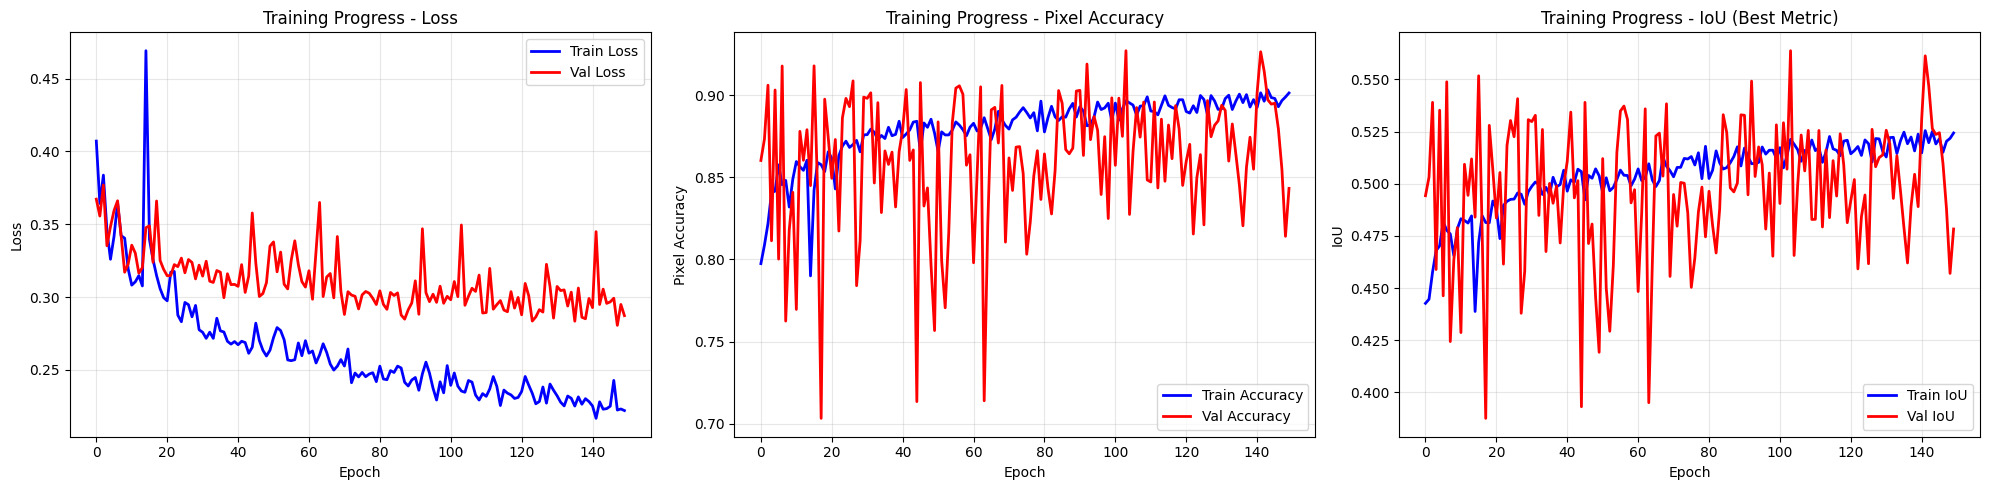
\includegraphics[width=0.9\linewidth]{figs/unet-bad-train.jpg}
  \caption{Training instability with BCE-only loss showing erratic convergence and suboptimal final performance}
  \label{fig:bad_training}
\end{figure}

The extreme class imbalance (97\% background pixels) caused the network to exploit the trivial solution of predicting background everywhere, achieving high pixel accuracy (0.97) but zero IoU. The loss function oscillated wildly as the network alternated between this degenerate solution and attempting to learn meaningful features. The combined Dice-Focal loss resolved this by directly optimising IoU-related metrics while down-weighting easy negative examples, leading to stable convergence and meaningful dead tree detection.

\paragraph{Performance Comparison: BCE vs. Combined Loss.}
Figure \ref{fig:loss_comparison} demonstrates the dramatic improvement achieved through our composite loss function:

\begin{figure}[htbp]
  \centering
  \begin{minipage}{0.47\linewidth}
    \centering
    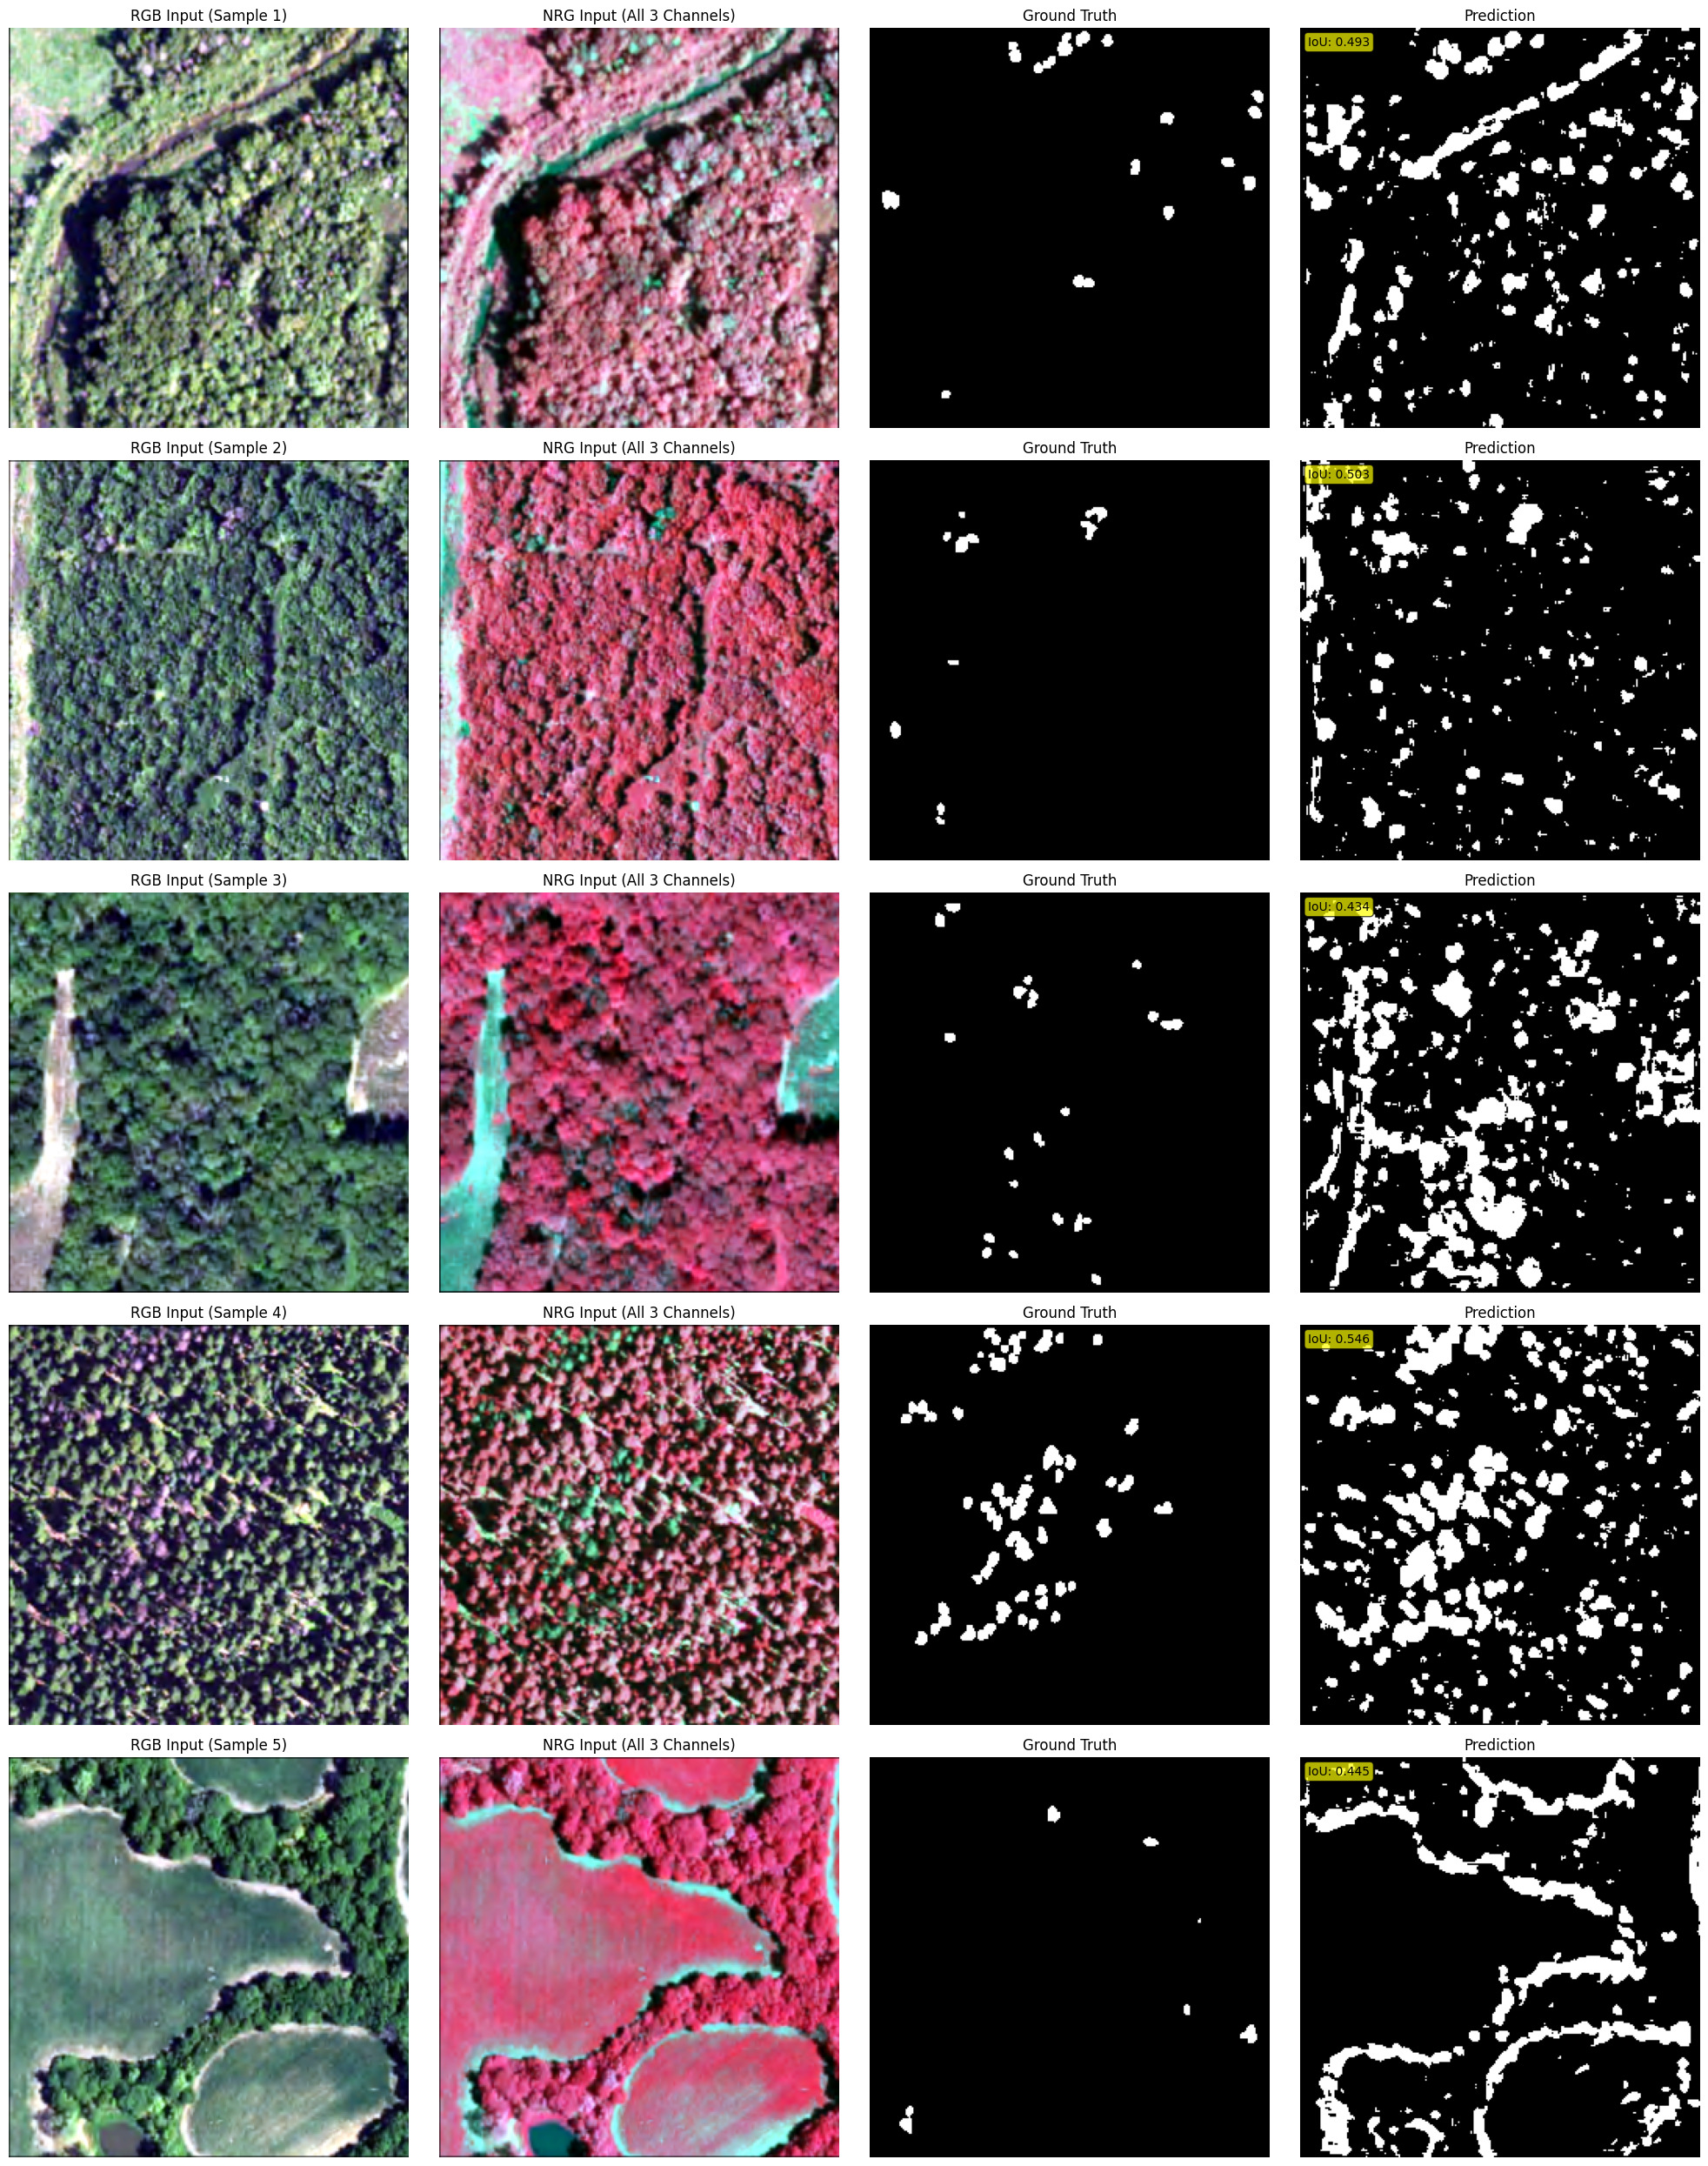
\includegraphics[width=0.9\linewidth]{figs/unet-bad-result-grid.jpg}
    \subcaption{BCE loss (IoU 0.12)}\label{fig:bad}
  \end{minipage}\hfill
  \begin{minipage}{0.47\linewidth}
    \centering
    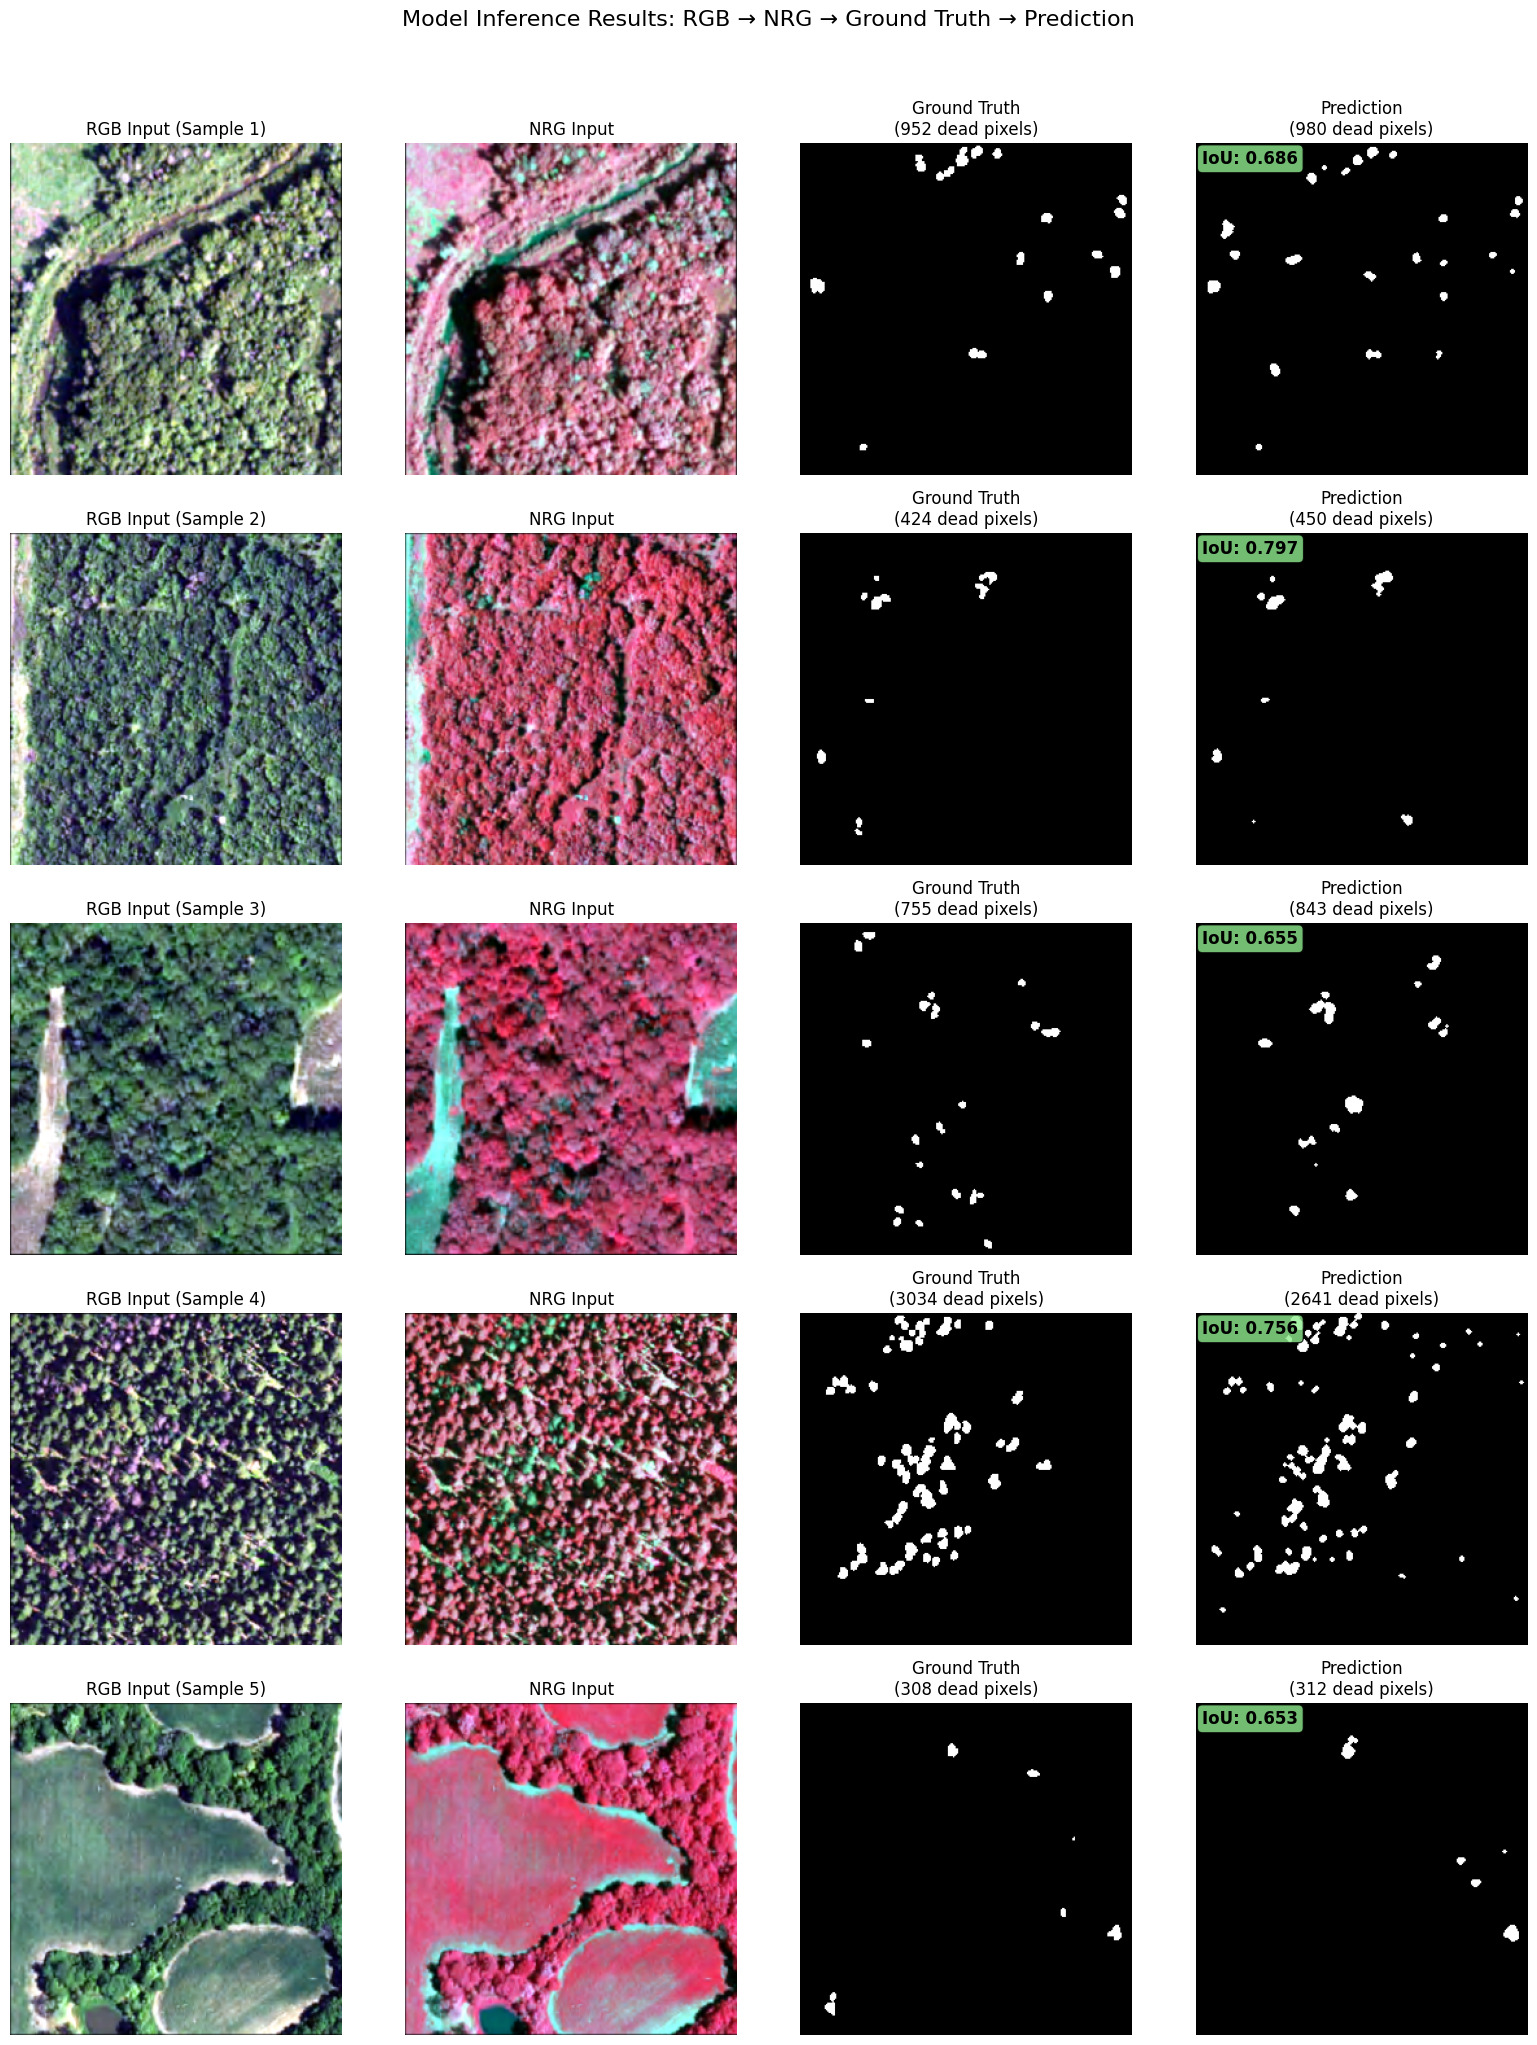
\includegraphics[width=0.9\linewidth]{figs/unet-good-result-grid.jpg}
    \subcaption{Dice + Focal (IoU 0.71)}\label{fig:good}
  \end{minipage}
  \caption{Segmentation quality comparison: BCE-only training produces sparse predictions (a) whereas the combined Dice–Focal loss yields coherent dead-tree masks (b).}
  \label{fig:loss_comparison}
\end{figure}

The BCE-only model produces sparse, disconnected predictions that fail to capture tree structures, while our combined loss generates coherent segmentations that accurately delineate dead tree boundaries.

\paragraph{Parameter Counts.}
The UNet implementation contains 31,042,434 parameters, distributed across the encoder-decoder hierarchy:

\begin{lstlisting}[language=Python]
print(f"UNET PARAMETERS: {sum(p.numel() for p in model.parameters()):,}")
> DEVICE: cuda
> UNET PARAMETERS: 31,034,690
\end{lstlisting}

This substantial parameter count demonstrates the robustness of this architecture compared to our other approaches. The simple CNN model, with only 4 convolutional layers and [32, 64, 128, 256] filters, contains approximately 2-3M parameters yet achieves only IoU = 0.286. Similarly, the DeepLabV3+ with CBAM model, built on a ResNet-18 backbone (~11M base parameters) with attention mechanisms and ASPP modules, totals roughly 15-18M parameters but reaches only IoU = 0.400.

The 31M-parameter UNet model however, achieves an IoU of 0.705—a 76\% improvement over CBAM and 146\% over the simple CNN! This performance gap justifies the increased parameter count: the encoder-decoder symmetry with skip connections requires substantial parameter investment, but enables precise boundary localisation that smaller networks cannot achieve. 

Furthermore, our model avoids the overfitting that plagued deeper CBAM variants (ResNet-50/101 showed no improvement), suggesting our parameter allocation is well-suited to the 355-image training set. 

\paragraph{Colour Jittering Abandonment.}
Initial data augmentation included colour jittering to improve generalisation:

\begin{lstlisting}[language=Python]
# orphaned augmentation approach
transforms.ColorJitter(brightness=0.2, contrast=0.2, saturation=0.2, hue=0.1)
\end{lstlisting}

We abandoned this pretty quick because it was a transformation that would only apply to the RGB channels and we wished to train on NIR too.
Colour jittering disrupts the spectral relationships so instead, we employed geometric augmentations (flips, rotations) that preserve spectral integrity while providing spatial generalisation.

\begin{lstlisting}[language=Python]
if augment:
    base_transforms.extend([
        T.RandomHorizontalFlip(p=0.5),
        T.RandomVerticalFlip(p=0.5),
        T.RandomRotation(10),
    ])
\end{lstlisting}


\paragraph{Final Architecture Performance.}
The optimised UNet architecture achieved robust performance across diverse test conditions, with post-processing providing consistent improvements. The 8-channel input pipeline, combined with the composite loss function and carefully selected augmentations, enabled effective dead tree segmentation despite significant class imbalance and complex spatial structures. The final IoU of 0.7078 represents a substantial improvement over baseline approaches and demonstrates the value of domain-specific architectural choices in challenging segmentation tasks.
